\documentclass{ctexart}
\usepackage{graphicx}
\usepackage{caption}
\usepackage{float}
\usepackage{amsmath}
\usepackage{fancyhdr}
\usepackage{xunicode-addon}
\usepackage{booktabs}
\usepackage{hyperref}
\usepackage[a4paper,hmargin=1.25in,vmargin=1in]{geometry}
% !TeX program = xelatex
\title{\begin{figure}[H]
	\centering 
	\includegraphics[height=7cm,width=14cm]{E:/Pictures/中科大.jpg}
	\end{figure}\Huge\textbf{Lab 5}\\\huge{}}
\date{}
\punctstyle{banjiao} 
\pagestyle{fancy}
	\fancyhead[C]{\LARGE\textbf{Report 5}}
	\fancyhead[L]{}
	\fancyhead[R]{}
	\fancyfoot[C]{\thepage}
\begin{document}
	\maketitle
	\thispagestyle{empty}
	
	\[\makebox{\Large{姓名:\underline{\makebox[5cm]{高茂航}}}}\]
	
    \[\makebox{\Large{学号:\underline{\makebox[5cm]{PB22061161}}}}\]
	
	$$\makebox{\Large{日期:\underline{\makebox[5cm]{2024.5.26}}}}$$
	
	\clearpage

	\pagenumbering{arabic}
	\section{Data preprocessing}
	数据预处理过程基本和lab3、lab4相同,主要区别是把数据集分为特征矩阵X和标签向量y,并
	用$LabelEncoder().fit\_transform()$把X,y转为数字索引以便于knn等算法的处理。
	值得注意的是,在lab4中我们将属性列用在整个表中的数字索引替换,
	而在这次实验中为了在分类时便于区分每一列,将每列各属性值替换为本列中的数字索引。

	本次实验也尝试了按7:1:2的比例划分训练集/验证集/测试集,
	但主要是使用k折交叉验证法划分训练集/测试集。
	\section{Algorithm Description}
	本次实验尝试了逻辑回归、决策树、随机森林、支持向量机、knn、神经网络等分类算法,但进行调参的主要是随机森林和决策树。
	此外,还尝试使用了PCA进行降维和数个算法的集成学习。各算法原理简述如下:
	\subsection{Logistic Regression}
	逻辑回归是一种统计模型,它使用逻辑函数对二元因变量进行建模,广泛用于二元分类问题。
	主要思想是:根据现有数据对分类边界线建立回归公式,以此进行分类。这个模型的输出值自然地落在0和1之间。逻辑回归不仅可以用于二元分类,还可以用于多元分类。

	\subsection{Random Forest}
	随机森林是一种集成学习方法,它通过在训练时构建多个决策树,并输出类别(分类)或个别树的平均预测(回归)的模式来操作。
	随机森林的工作原理是,每个决策树都在一个随机子集上进行训练,然后对结果进行投票,对于分类问题,结果是投票最多的类别,对于回归问题,结果是平均预测值。
	
	随机森林通过组合多个决策树的预测来减少过拟合的可能性,提高泛化能力,且由于随机性,它能够有效地处理非线性和高维数据,而且不需要过多的参数调整就可以给出很好的结果。
随机森林的另一个优点是,它可以用于评估特征的重要性,这在解释数据时非常有用。


	\subsection{Decision Tree}
	决策树是一种监督学习算法,主要用于分类问题,但也可以解决回归问题。
	它是一种树形结构,其中每个内部节点代表一个特征(或属性),每个分支代表一个决策规则,每个叶节点代表一个结果。
	决策树的构建过程是一个递归过程,首先选择一个最优特征,根据这个特征分割数据,然后对子集数据再次进行这个过程,直到满足某些停止条件(如所有实例都属于同一类别,或者没有更多特征)。

决策树的主要优点是简单易懂,可解释性强。通过观察决策树,我们可以理解模型的决策过程。此外,决策树不需要对数据进行太多预处理,不需要进行归一化,也不需要处理缺失值。


	\subsection{K-Nearest Neighbors}
	K-最近邻是一种基于实例的学习或者是局部近似和将所有计算推迟到函数评估的惰性学习。
工作原理是:对于一个待预测的数据点,算法会查找训练集中与其最近的K个邻居,然后根据这些邻居的类别,通过投票等方式来预测该数据点的类别。其中,K是一个用户定义的参数。

K-最近邻算法简单易懂,易于实现,无需训练阶段,适合对稀有事件进行分类,以及解决多分类问题。但是,K-最近邻算法计算量大,特别是当数据集很大时,需要计算待预测点与所有训练数据点的距离,计算复杂度高。此外,K-最近邻算法对于特征的缩放和异常值敏感。
	\subsection{Multi-Layer Perceptron}
	多层感知器是一种前馈神经网络,包含至少三层(输入层、隐藏层和输出层)的节点。每一层都完全连接到下一层的节点。在MLP中,信息从输入层开始,通过隐藏层,最后到达输出层。
	多层感知器可以处理复杂的非线性分类问题,是深度学习的基础。然而,它也有一些缺点,比如可能会遇到过拟合问题,训练过程可能会比较慢,以及需要手动选择合适的网络结构
	\subsection{Support Vector Machine}
	支持向量机是一种监督学习模型,主要用于分类和回归分析。在二分类问题中,支持向量机的基本思想是找到一个超平面,使得两个类别的样本在该超平面两侧,且距离超平面最近的样本点(即支持向量)到超平面的距离(即间隔)最大。
对于线性不可分的数据,支持向量机通过引入核函数,将原始数据映射到一个更高维的空间,使得数据在新的空间中变得线性可分。

支持向量机的一个优点是,它只依赖于支持向量,而不是全部数据。这使得模型更加稳健,不容易受到噪声数据的影响。然而,对于大规模数据,支持向量机的训练过程可能会比较耗时。
	\subsection{Ensemble Learning}
	集成学习是一种机器学习范式,其主要目标是通过组合多个弱学习器,提高预测的准确性或稳定性,主要方法包括Bagging、Boosting和Stacking。
	\subsection{PCA}
	主成分分析通过线性变换将一组可能相关的变量转化为一组线性无关的变量(主成分),主要用于数据的降维,可以有效地去除数据的噪声,提取数据的主要特征。但是,PCA是一种线性方法,可能无法有效地处理非线性数据。此外,PCA假设主成分是正交的,这可能不适用于所有数据。
    \section{Lab3's Data(run1.ipynb)}
	\subsection{Process}
    首先使用随机森林和k折检验法,没有调参时分类准确度就达到了0.9589285714285716,已经是非常高的水平了。
	接着尝试找到$n\_estimators$的最优值,发现在$n\_estimators=51$时分类准确度最高,为0.9660714285714285。
	随后调整$max\_depth$,发现在$max\_depth=7$时分类准确度最高,为0.9678571428571429。
	还调整了$max\_features$,发现$max\_features=6$时准确率能达到0.968421052631579。
	根据上述找到的最优值,定义一个参数网络依次计算,得到$max\_depth=7, max\_features=5, n\_estimators=45$时准确率最高,能达到0.9696428571428571。
	
	接下来定义参数网络对逻辑回归进行调参,发现$C=100, penalty=l2, solver=newton-cg$时准确率能达到0.9625,略低于随机森林。
	还尝试了对决策树进行调参,发现准确率能达到0.9517857142857142,较前面更低。

	最后,我还尝试了PCA降维、只保留X中与y相关性较强的列、集成学习等方法,但效果都大差不差,位于0.95-0.96间,没能超过0.97。


\subsection{Results}
以下展示了按7:1:2的比例划分训练集/验证集/测试集且未调参时几种算法的结果:
\begin{figure}[H]
	\centering 
	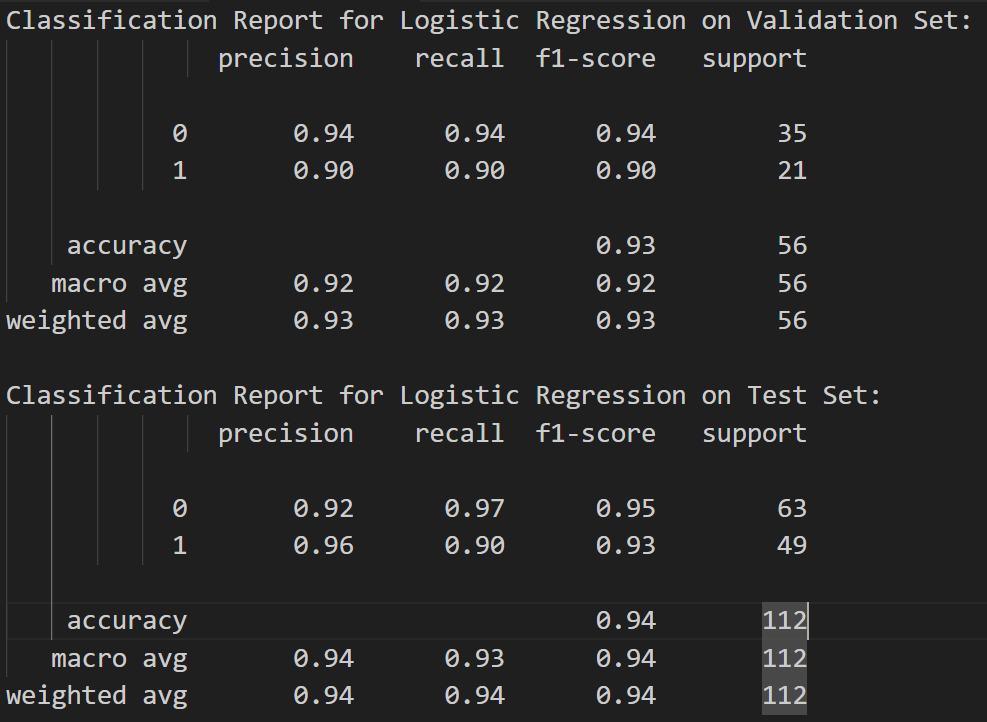
\includegraphics[height=7cm,width=10cm]{1.png}
	\end{figure}
	\begin{figure}[H]
		\centering 
		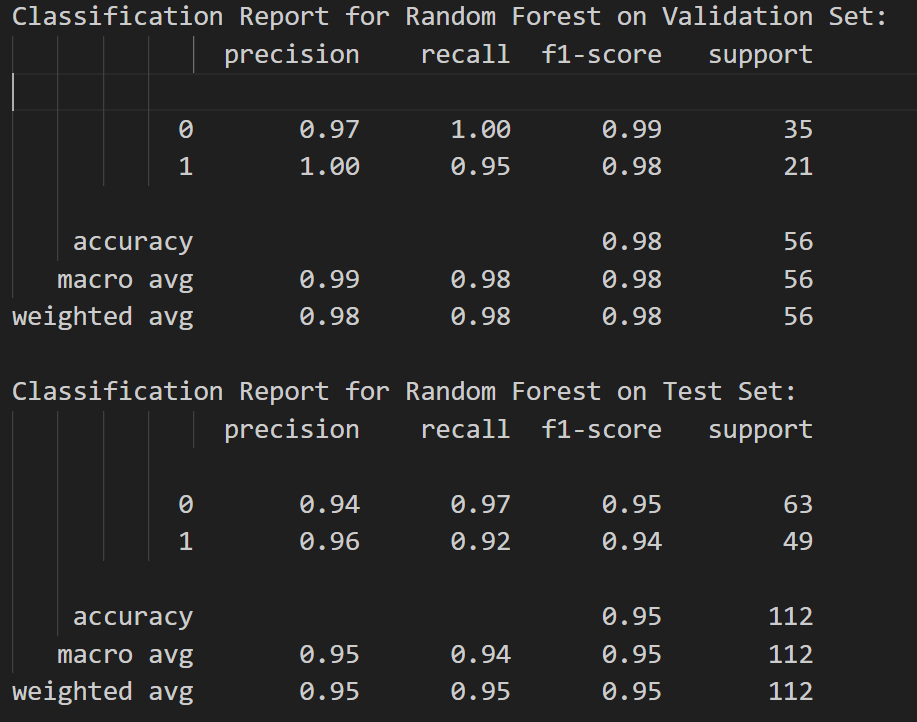
\includegraphics[height=7cm,width=10cm]{2.png}
		\end{figure}
		\begin{figure}[H]
			\centering 
			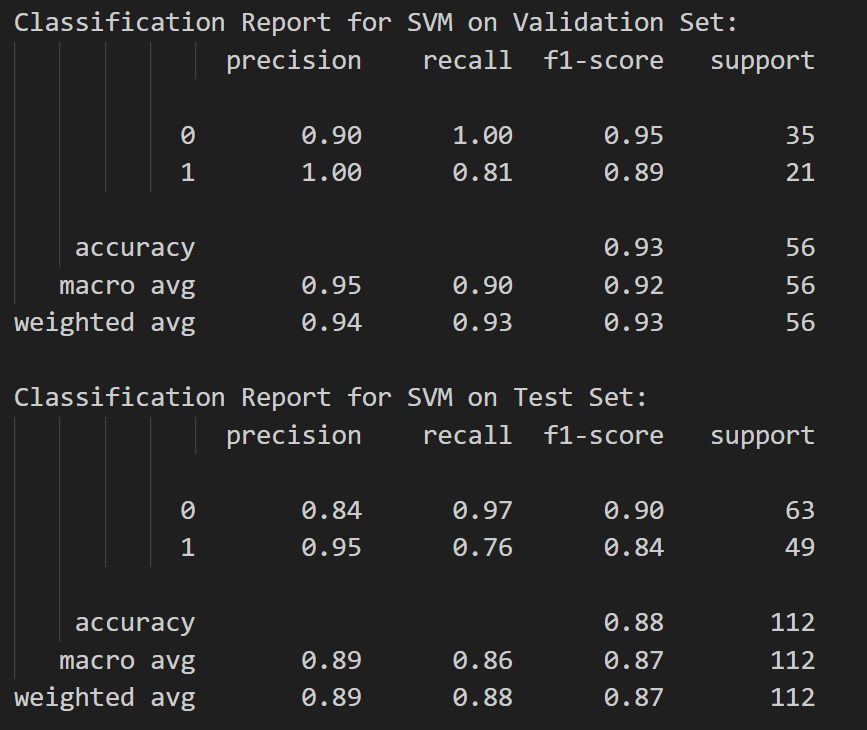
\includegraphics[height=7cm,width=10cm]{3.png}
			\end{figure}
			\begin{figure}[H]
				\centering 
				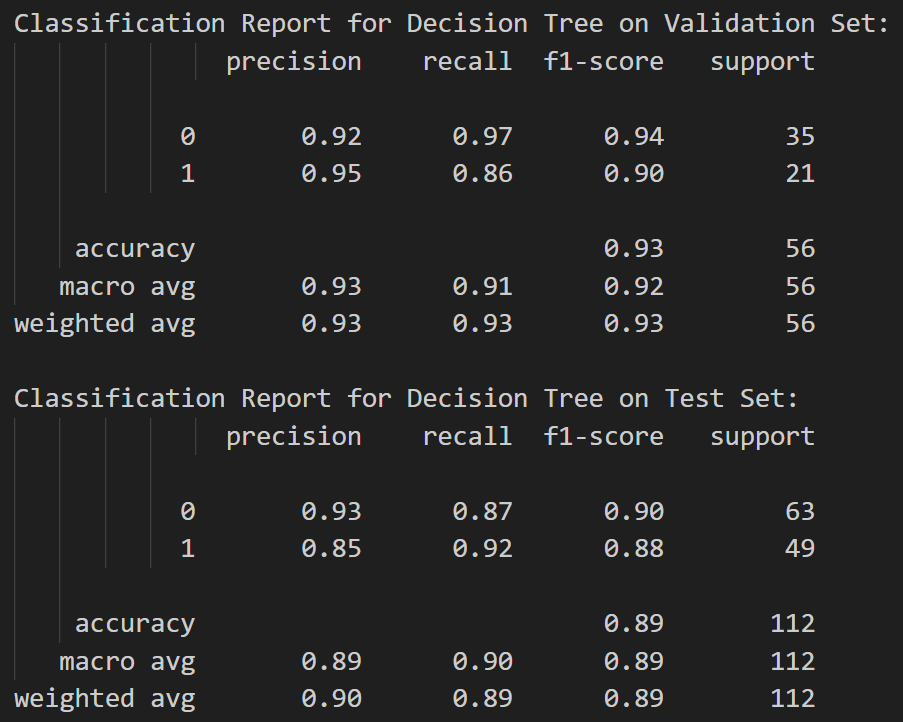
\includegraphics[height=7cm,width=10cm]{4.png}
				\end{figure}
可见随机森林的分类效果最好,但存在一定的过拟合现象,逻辑回归次之,决策树和支持向量机分类效果最差,
且过拟合现象严重,但由于未调参,因此还无法严格地比较。综合3.1的分析过程,目前认为随机森林的分类效果最好,但经过调参提高效果不明显。

    \section{Lab4's Data(run2.ipynb)}
    \subsection{Process}
	首先使用随机森林和k折检验法,没有调参时分类准确度为0.6858465608465607。
	
	由于在lab4中我们发现irradiat、node-caps、inv-nodes
	三列中有因素与不复发强关联,因此我想保留只这三列,但发现效果并不好,准确率只有0.6665343915343915。

	接下来和3.1类似,也是依次分别调整随机森林的$n\_estimators$、$max\_depth$、$max\_features$、$min\_samples\_split$、$min\_samples\_leaf$,
	发现$min\_samples\_leaf=18$时准确率最高,能达到0.7690476190476191,其他准确率在0.65-0.75之间。
	接着用参数网络分别对随机森林和决策树进行整体调参,发现决策树的准确率能达到最优,为0.7794973544973545。
	随后我还试图用皮尔逊相关系数判断X每列和y的相关性,但发现相关系数都非常低,另外我也尝试了PCA降维、神经网络、集成学习,但都没能超过0.78。
	\subsection{Results}
以下展示了按7:1:2的比例划分训练集/验证集/测试集且未调参时几种算法的结果:

\begin{figure}[H]
	\centering 
	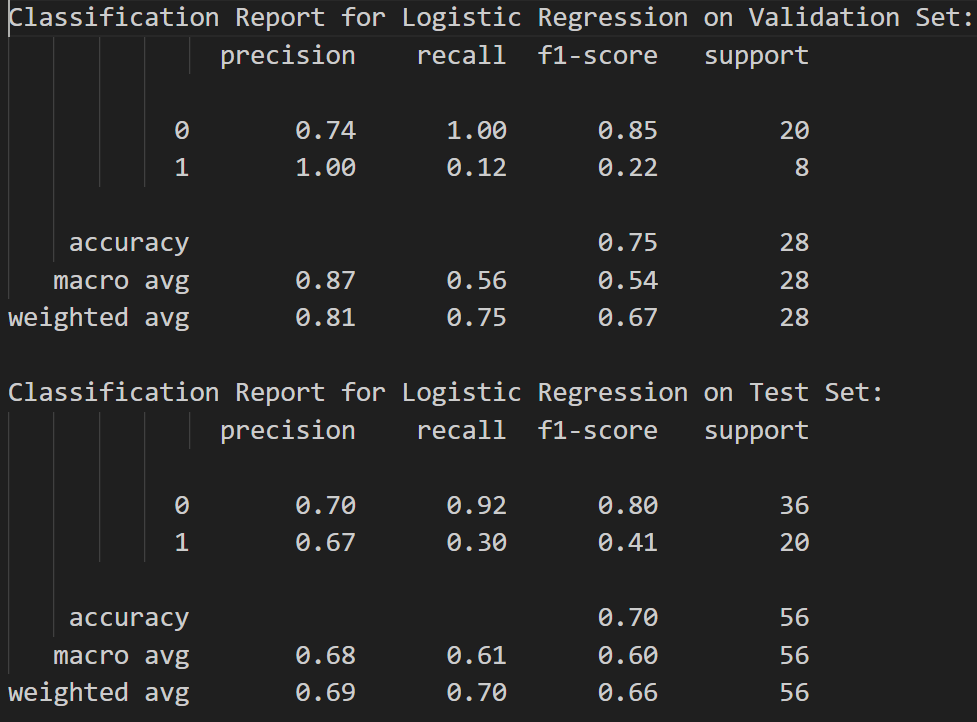
\includegraphics[height=7cm,width=10cm]{5.png}
	\end{figure}
	\begin{figure}[H]
		\centering 
		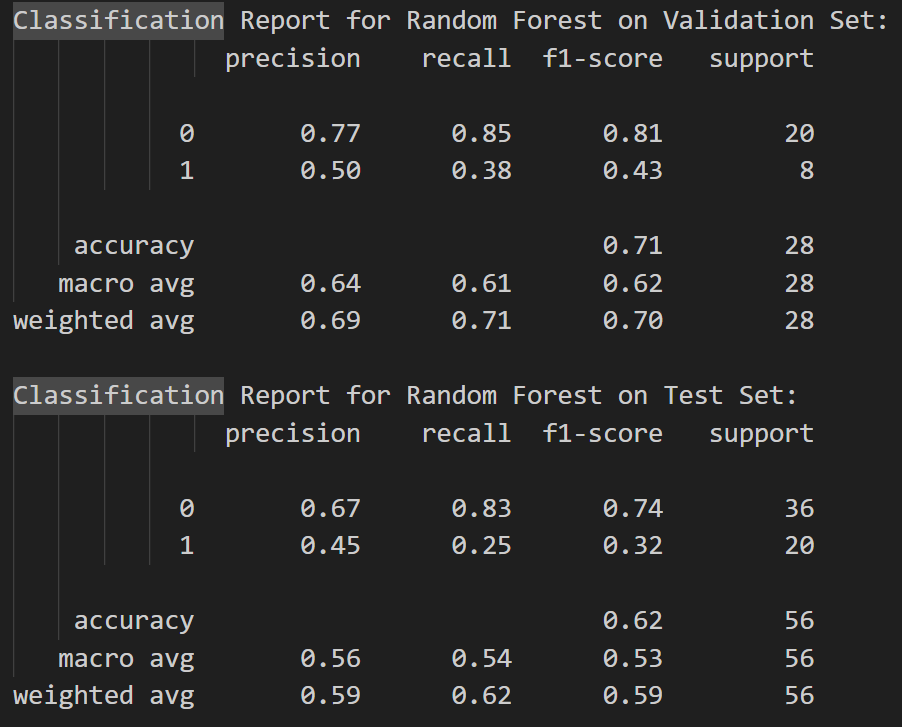
\includegraphics[height=7cm,width=10cm]{6.png}
		\end{figure}
		\begin{figure}[H]
			\centering 
			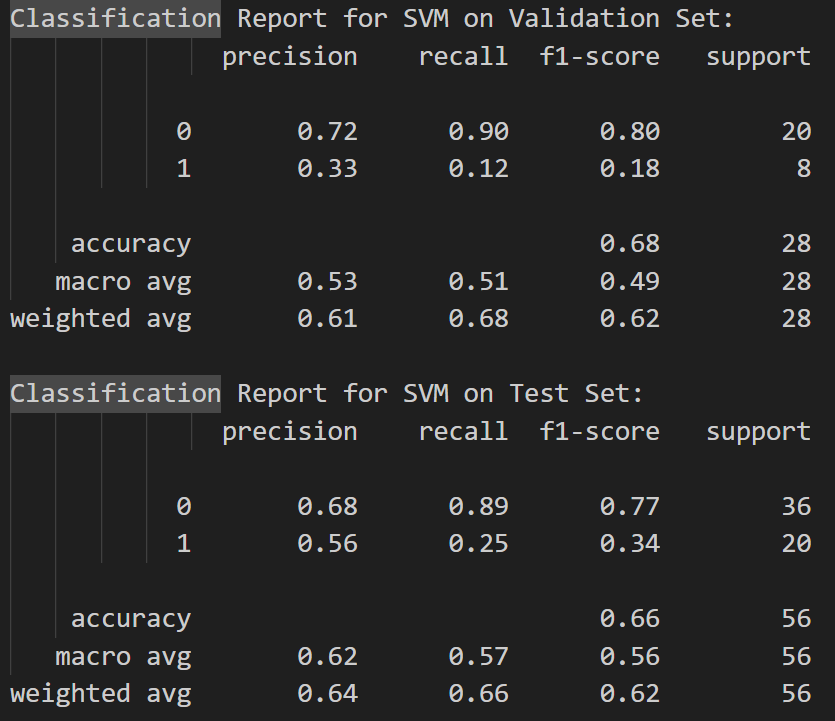
\includegraphics[height=7cm,width=10cm]{7.png}
			\end{figure}
			\begin{figure}[H]
				\centering 
				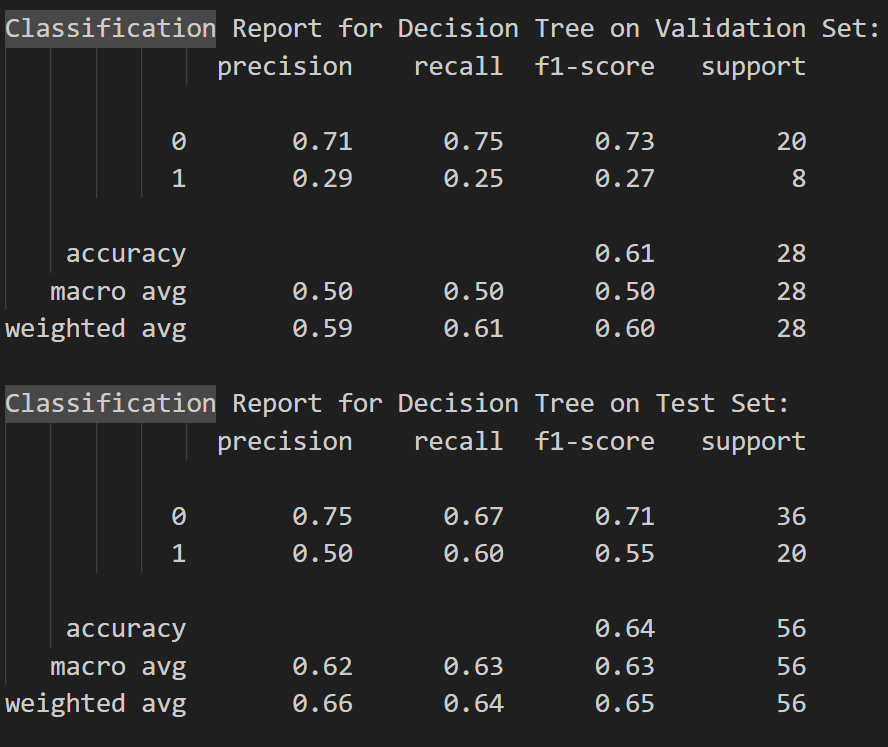
\includegraphics[height=7cm,width=10cm]{8.png}
				\end{figure}
				\begin{figure}[H]
					\centering 
					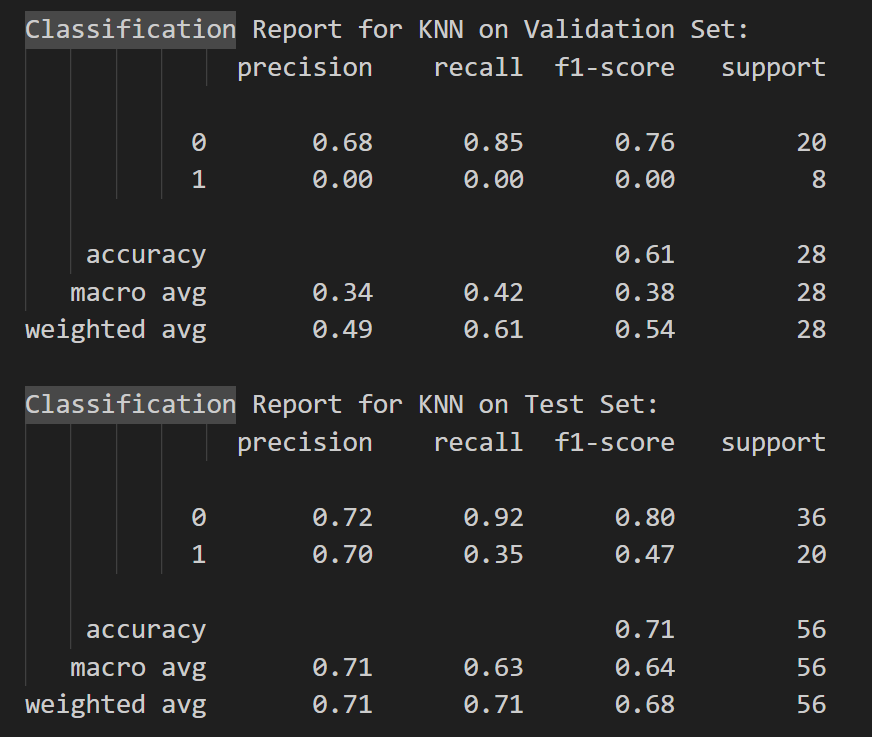
\includegraphics[height=7cm,width=10cm]{9.png}
					\end{figure}
			可见在没调参时各算法对应指标的效果互有差异,但在测试集上的准确率都在0.6-0.7之间,且都有一定的过拟合现象,
			没有发现哪个算法有明显优势。
			综合4.1的分析,目前只能认为决策树整体调参后效果最优,准确率能达到0.779,较未调参时有一定提高,但不算太明显。
   \section{Conclusion}	
   通过这次实验,我进一步加深了对数据分析整体过程的理解,并尝试了多种特征工程和分类算法,运用了课堂学到的知识,
   也了解到了调参的方法。但就结果而言,个人不太满意,因为lab3的数据集不用处理时准确率已经非常高了,没能找到更好的改进办法。
   而对于lab4的数据集,尝试了多种算法和调参方式后准确率有一定提高,但还没能达到0.8,可能是对数据集的特征认识不够深刻,
   还需在将来的学习过程中积累预处理和特征工程的经验,以达到更好的效果。
   \section{References}
   1.\href{https://scikit-learn.org/stable/}{Scikit-learn机器学习库官方网站}

2.\href{https://www.kaggle.com/datasets/uciml/breast-cancer-wisconsin-data}{Kaggle乳腺癌数据集}

3.\href{https://zhuanlan.zhihu.com/p/30504716}{机器学习利器——决策树和随机森林}

4.\href{https://zhuanlan.zhihu.com/p/74874291}{【机器学习】逻辑回归(非常详细)}

5.\href{https://www.zhihu.com/tardis/zm/art/31886934?source_id=1003}{支持向量机(SVM)——原理篇}

6.\href{https://zhuanlan.zhihu.com/p/110913279}{机器学习算法之——K最近邻(k-Nearest Neighbor,KNN)分类算法原理讲解}
\end{document}